% =====================================================================
% figF  — R/ggplot2 -> tikzDevice (parallel to ../figures-tex/figF_sequential.tex)
% Canonical-JSON-only. Regenerate: Rscript figures-r/make_figures.R
% Provenance (JSON path :: field = plotted value), one line per series:
% SOURCE: results/SEQ_analysis_L12_4stream.json :: per_stream[0].survival_curve[10].frac_survived = 0.5000
% SOURCE: results/SEQ_analysis_L12_4stream.json :: per_stream[0].survival_curve[20].frac_survived = 0.3500
% SOURCE: results/SEQ_analysis_L12_4stream.json :: per_stream[0].survival_curve[30].frac_survived = 0.3667
% SOURCE: results/SEQ_analysis_L12_4stream.json :: per_stream[0].survival_curve[40].frac_survived = 0.2250
% SOURCE: results/SEQ_analysis_L12_4stream.json :: per_stream[0].survival_curve[50].frac_survived = 0.1000
% SOURCE: results/SEQ_analysis_L12_4stream.json :: per_stream[1].survival_curve[10].frac_survived = 0.6000
% SOURCE: results/SEQ_analysis_L12_4stream.json :: per_stream[1].survival_curve[20].frac_survived = 0.3000
% SOURCE: results/SEQ_analysis_L12_4stream.json :: per_stream[1].survival_curve[30].frac_survived = 0.3667
% SOURCE: results/SEQ_analysis_L12_4stream.json :: per_stream[1].survival_curve[40].frac_survived = 0.4000
% SOURCE: results/SEQ_analysis_L12_4stream.json :: per_stream[1].survival_curve[50].frac_survived = 0.1400
% SOURCE: results/SEQ_analysis_L12_4stream.json :: per_stream[2].survival_curve[10].frac_survived = 0.6000
% SOURCE: results/SEQ_analysis_L12_4stream.json :: per_stream[2].survival_curve[20].frac_survived = 0.6000
% SOURCE: results/SEQ_analysis_L12_4stream.json :: per_stream[2].survival_curve[30].frac_survived = 0.7000
% SOURCE: results/SEQ_analysis_L12_4stream.json :: per_stream[2].survival_curve[40].frac_survived = 0.3500
% SOURCE: results/SEQ_analysis_L12_4stream.json :: per_stream[2].survival_curve[50].frac_survived = 0.4200
% SOURCE: results/SEQ_analysis_L12_4stream.json :: per_stream[3].survival_curve[10].frac_survived = 0.4000
% SOURCE: results/SEQ_analysis_L12_4stream.json :: per_stream[3].survival_curve[20].frac_survived = 0.5000
% SOURCE: results/SEQ_analysis_L12_4stream.json :: per_stream[3].survival_curve[30].frac_survived = 0.3333
% SOURCE: results/SEQ_analysis_L12_4stream.json :: per_stream[3].survival_curve[40].frac_survived = 0.1750
% SOURCE: results/SEQ_analysis_L12_4stream.json :: per_stream[3].survival_curve[50].frac_survived = 0.3600
% SOURCE: results/SEQ_analysis_L12_4stream.json :: per_stream[0].position_fragility.rho_position_vs_survival = 0.3118
% SOURCE: results/SEQ_analysis_L12_4stream.json :: per_stream[1].position_fragility.rho_position_vs_survival = 0.2017
% SOURCE: results/SEQ_analysis_L12_4stream.json :: per_stream[2].position_fragility.rho_position_vs_survival = 0.4816
% SOURCE: results/SEQ_analysis_L12_4stream.json :: per_stream[3].position_fragility.rho_position_vs_survival = 0.5139
% SOURCE: results/SEQ_analysis_L12_4stream.json :: pooled.position_fragility.rho_position_vs_survival = 0.3716
% =====================================================================
% !TEX encoding = UTF-8 Unicode
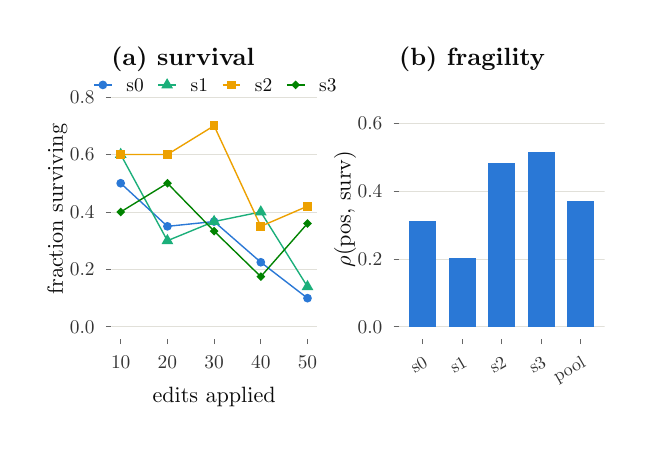
\begin{tikzpicture}[x=1pt,y=1pt]
\definecolor{fillColor}{RGB}{255,255,255}
\path[use as bounding box,fill=fillColor,fill opacity=0.00] (0,0) rectangle (218.98,144.54);
\begin{scope}
\path[clip] (  0.00,  0.00) rectangle (218.98,144.54);
\definecolor{drawColor}{RGB}{255,255,255}
\definecolor{fillColor}{RGB}{255,255,255}

\path[draw=drawColor,line width= 0.6pt,line join=round,line cap=round,fill=fillColor] (  0.00, -0.00) rectangle (218.98,144.54);
\end{scope}
\begin{scope}
\path[clip] (  5.50,  5.50) rectangle (109.49,139.04);
\definecolor{fillColor}{RGB}{255,255,255}

\path[fill=fillColor] (  5.50,  5.50) rectangle (109.49,139.04);
\end{scope}
\begin{scope}
\path[clip] (109.49,  5.50) rectangle (213.48,139.04);
\definecolor{fillColor}{RGB}{255,255,255}

\path[fill=fillColor] (109.49,  5.50) rectangle (213.48,139.04);
\end{scope}
\begin{scope}
\path[clip] ( 30.24, 32.15) rectangle (104.49,125.82);
\definecolor{drawColor}{RGB}{225,224,217}

\path[draw=drawColor,line width= 0.3pt,line join=round] ( 30.24, 36.41) --
	(104.49, 36.41);

\path[draw=drawColor,line width= 0.3pt,line join=round] ( 30.24, 57.18) --
	(104.49, 57.18);

\path[draw=drawColor,line width= 0.3pt,line join=round] ( 30.24, 77.95) --
	(104.49, 77.95);

\path[draw=drawColor,line width= 0.3pt,line join=round] ( 30.24, 98.72) --
	(104.49, 98.72);

\path[draw=drawColor,line width= 0.3pt,line join=round] ( 30.24,119.48) --
	(104.49,119.48);
\definecolor{drawColor}{RGB}{42,120,214}

\path[draw=drawColor,line width= 0.5pt,line join=round] ( 33.61, 88.33) --
	( 50.49, 72.75) --
	( 67.36, 74.49) --
	( 84.24, 59.77) --
	(101.11, 46.79);
\definecolor{drawColor}{RGB}{27,175,122}

\path[draw=drawColor,line width= 0.5pt,line join=round] ( 33.61, 98.72) --
	( 50.49, 67.56) --
	( 67.36, 74.49) --
	( 84.24, 77.95) --
	(101.11, 50.95);
\definecolor{drawColor}{RGB}{237,161,0}

\path[draw=drawColor,line width= 0.5pt,line join=round] ( 33.61, 98.72) --
	( 50.49, 98.72) --
	( 67.36,109.10) --
	( 84.24, 72.75) --
	(101.11, 80.02);
\definecolor{drawColor}{RGB}{0,131,0}

\path[draw=drawColor,line width= 0.5pt,line join=round] ( 33.61, 77.95) --
	( 50.49, 88.33) --
	( 67.36, 71.02) --
	( 84.24, 54.58) --
	(101.11, 73.79);
\definecolor{fillColor}{RGB}{42,120,214}

\path[fill=fillColor] ( 33.61, 88.33) circle (  1.58);

\path[fill=fillColor] ( 50.49, 72.75) circle (  1.58);

\path[fill=fillColor] ( 67.36, 74.49) circle (  1.58);

\path[fill=fillColor] ( 84.24, 59.77) circle (  1.58);

\path[fill=fillColor] (101.11, 46.79) circle (  1.58);
\definecolor{fillColor}{RGB}{27,175,122}

\path[fill=fillColor] ( 33.61,101.17) --
	( 35.74, 97.49) --
	( 31.49, 97.49) --
	cycle;

\path[fill=fillColor] ( 50.49, 70.01) --
	( 52.61, 66.34) --
	( 48.37, 66.34) --
	cycle;

\path[fill=fillColor] ( 67.36, 76.94) --
	( 69.49, 73.26) --
	( 65.24, 73.26) --
	cycle;

\path[fill=fillColor] ( 84.24, 80.40) --
	( 86.36, 76.72) --
	( 82.12, 76.72) --
	cycle;

\path[fill=fillColor] (101.11, 53.40) --
	(103.24, 49.72) --
	( 98.99, 49.72) --
	cycle;
\definecolor{fillColor}{RGB}{237,161,0}

\path[fill=fillColor] ( 32.04, 97.14) --
	( 35.19, 97.14) --
	( 35.19,100.29) --
	( 32.04,100.29) --
	cycle;

\path[fill=fillColor] ( 48.91, 97.14) --
	( 52.07, 97.14) --
	( 52.07,100.29) --
	( 48.91,100.29) --
	cycle;

\path[fill=fillColor] ( 65.79,107.52) --
	( 68.94,107.52) --
	( 68.94,110.68) --
	( 65.79,110.68) --
	cycle;

\path[fill=fillColor] ( 82.66, 71.18) --
	( 85.82, 71.18) --
	( 85.82, 74.33) --
	( 82.66, 74.33) --
	cycle;

\path[fill=fillColor] ( 99.54, 78.45) --
	(102.69, 78.45) --
	(102.69, 81.60) --
	( 99.54, 81.60) --
	cycle;
\definecolor{fillColor}{RGB}{0,131,0}

\path[fill=fillColor] ( 32.04, 77.95) --
	( 33.61, 79.52) --
	( 35.19, 77.95) --
	( 33.61, 76.37) --
	cycle;

\path[fill=fillColor] ( 48.91, 88.33) --
	( 50.49, 89.91) --
	( 52.07, 88.33) --
	( 50.49, 86.75) --
	cycle;

\path[fill=fillColor] ( 65.79, 71.02) --
	( 67.36, 72.60) --
	( 68.94, 71.02) --
	( 67.36, 69.44) --
	cycle;

\path[fill=fillColor] ( 82.66, 54.58) --
	( 84.24, 56.16) --
	( 85.82, 54.58) --
	( 84.24, 53.01) --
	cycle;

\path[fill=fillColor] ( 99.54, 73.79) --
	(101.11, 75.37) --
	(102.69, 73.79) --
	(101.11, 72.22) --
	cycle;
\end{scope}
\begin{scope}
\path[clip] (  0.00,  0.00) rectangle (218.98,144.54);
\definecolor{drawColor}{gray}{0.20}

\node[text=drawColor,anchor=base east,inner sep=0pt, outer sep=0pt, scale=  0.70] at ( 24.19, 34.13) {0.0};

\node[text=drawColor,anchor=base east,inner sep=0pt, outer sep=0pt, scale=  0.70] at ( 24.19, 54.90) {0.2};

\node[text=drawColor,anchor=base east,inner sep=0pt, outer sep=0pt, scale=  0.70] at ( 24.19, 75.67) {0.4};

\node[text=drawColor,anchor=base east,inner sep=0pt, outer sep=0pt, scale=  0.70] at ( 24.19, 96.44) {0.6};

\node[text=drawColor,anchor=base east,inner sep=0pt, outer sep=0pt, scale=  0.70] at ( 24.19,117.21) {0.8};
\end{scope}
\begin{scope}
\path[clip] (  0.00,  0.00) rectangle (218.98,144.54);
\definecolor{drawColor}{gray}{0.40}

\path[draw=drawColor,line width= 0.3pt,line join=round] ( 28.24, 36.41) --
	( 30.24, 36.41);

\path[draw=drawColor,line width= 0.3pt,line join=round] ( 28.24, 57.18) --
	( 30.24, 57.18);

\path[draw=drawColor,line width= 0.3pt,line join=round] ( 28.24, 77.95) --
	( 30.24, 77.95);

\path[draw=drawColor,line width= 0.3pt,line join=round] ( 28.24, 98.72) --
	( 30.24, 98.72);

\path[draw=drawColor,line width= 0.3pt,line join=round] ( 28.24,119.48) --
	( 30.24,119.48);
\end{scope}
\begin{scope}
\path[clip] (  0.00,  0.00) rectangle (218.98,144.54);
\definecolor{drawColor}{gray}{0.40}

\path[draw=drawColor,line width= 0.3pt,line join=round] ( 33.61, 30.15) --
	( 33.61, 32.15);

\path[draw=drawColor,line width= 0.3pt,line join=round] ( 50.49, 30.15) --
	( 50.49, 32.15);

\path[draw=drawColor,line width= 0.3pt,line join=round] ( 67.36, 30.15) --
	( 67.36, 32.15);

\path[draw=drawColor,line width= 0.3pt,line join=round] ( 84.24, 30.15) --
	( 84.24, 32.15);

\path[draw=drawColor,line width= 0.3pt,line join=round] (101.11, 30.15) --
	(101.11, 32.15);
\end{scope}
\begin{scope}
\path[clip] (  0.00,  0.00) rectangle (218.98,144.54);
\definecolor{drawColor}{gray}{0.20}

\node[text=drawColor,anchor=base,inner sep=0pt, outer sep=0pt, scale=  0.70] at ( 33.61, 21.54) {10};

\node[text=drawColor,anchor=base,inner sep=0pt, outer sep=0pt, scale=  0.70] at ( 50.49, 21.54) {20};

\node[text=drawColor,anchor=base,inner sep=0pt, outer sep=0pt, scale=  0.70] at ( 67.36, 21.54) {30};

\node[text=drawColor,anchor=base,inner sep=0pt, outer sep=0pt, scale=  0.70] at ( 84.24, 21.54) {40};

\node[text=drawColor,anchor=base,inner sep=0pt, outer sep=0pt, scale=  0.70] at (101.11, 21.54) {50};
\end{scope}
\begin{scope}
\path[clip] (  0.00,  0.00) rectangle (218.98,144.54);
\definecolor{drawColor}{RGB}{11,11,11}

\node[text=drawColor,anchor=base,inner sep=0pt, outer sep=0pt, scale=  0.80] at ( 67.36,  9.23) {edits applied};
\end{scope}
\begin{scope}
\path[clip] (  0.00,  0.00) rectangle (218.98,144.54);
\definecolor{drawColor}{RGB}{11,11,11}

\node[text=drawColor,rotate= 90.00,anchor=base,inner sep=0pt, outer sep=0pt, scale=  0.80] at ( 12.71, 78.98) {fraction surviving};
\end{scope}
\begin{scope}
\path[clip] (  0.00,  0.00) rectangle (218.98,144.54);
\definecolor{drawColor}{RGB}{42,120,214}

\path[draw=drawColor,line width= 0.5pt,line join=round] ( 23.97,123.85) -- ( 30.37,123.85);
\definecolor{fillColor}{RGB}{42,120,214}

\path[fill=fillColor] ( 27.17,123.85) circle (  1.58);
\end{scope}
\begin{scope}
\path[clip] (  0.00,  0.00) rectangle (218.98,144.54);
\definecolor{drawColor}{RGB}{27,175,122}

\path[draw=drawColor,line width= 0.5pt,line join=round] ( 47.19,123.85) -- ( 53.59,123.85);
\definecolor{fillColor}{RGB}{27,175,122}

\path[fill=fillColor] ( 50.39,126.31) --
	( 52.51,122.63) --
	( 48.27,122.63) --
	cycle;
\end{scope}
\begin{scope}
\path[clip] (  0.00,  0.00) rectangle (218.98,144.54);
\definecolor{drawColor}{RGB}{237,161,0}

\path[draw=drawColor,line width= 0.5pt,line join=round] ( 70.41,123.85) -- ( 76.81,123.85);
\definecolor{fillColor}{RGB}{237,161,0}

\path[fill=fillColor] ( 72.04,122.28) --
	( 75.19,122.28) --
	( 75.19,125.43) --
	( 72.04,125.43) --
	cycle;
\end{scope}
\begin{scope}
\path[clip] (  0.00,  0.00) rectangle (218.98,144.54);
\definecolor{drawColor}{RGB}{0,131,0}

\path[draw=drawColor,line width= 0.5pt,line join=round] ( 93.64,123.85) -- (100.04,123.85);
\definecolor{fillColor}{RGB}{0,131,0}

\path[fill=fillColor] ( 95.26,123.85) --
	( 96.84,125.43) --
	( 98.41,123.85) --
	( 96.84,122.28) --
	cycle;
\end{scope}
\begin{scope}
\path[clip] (  0.00,  0.00) rectangle (218.98,144.54);
\definecolor{drawColor}{RGB}{11,11,11}

\node[text=drawColor,anchor=base west,inner sep=0pt, outer sep=0pt, scale=  0.70] at ( 35.67,121.58) {s0};
\end{scope}
\begin{scope}
\path[clip] (  0.00,  0.00) rectangle (218.98,144.54);
\definecolor{drawColor}{RGB}{11,11,11}

\node[text=drawColor,anchor=base west,inner sep=0pt, outer sep=0pt, scale=  0.70] at ( 58.89,121.58) {s1};
\end{scope}
\begin{scope}
\path[clip] (  0.00,  0.00) rectangle (218.98,144.54);
\definecolor{drawColor}{RGB}{11,11,11}

\node[text=drawColor,anchor=base west,inner sep=0pt, outer sep=0pt, scale=  0.70] at ( 82.11,121.58) {s2};
\end{scope}
\begin{scope}
\path[clip] (  0.00,  0.00) rectangle (218.98,144.54);
\definecolor{drawColor}{RGB}{11,11,11}

\node[text=drawColor,anchor=base west,inner sep=0pt, outer sep=0pt, scale=  0.70] at (105.34,121.58) {s3};
\end{scope}
\begin{scope}
\path[clip] (  0.00,  0.00) rectangle (218.98,144.54);
\definecolor{drawColor}{RGB}{11,11,11}

\node[text=drawColor,anchor=base west,inner sep=0pt, outer sep=0pt, scale=  0.90] at ( 30.24,130.84) {\bfseries (a) survival};
\end{scope}
\begin{scope}
\path[clip] (134.23, 32.15) rectangle (208.48,125.82);
\definecolor{drawColor}{RGB}{225,224,217}

\path[draw=drawColor,line width= 0.3pt,line join=round] (134.23, 36.41) --
	(208.48, 36.41);

\path[draw=drawColor,line width= 0.3pt,line join=round] (134.23, 60.96) --
	(208.48, 60.96);

\path[draw=drawColor,line width= 0.3pt,line join=round] (134.23, 85.50) --
	(208.48, 85.50);

\path[draw=drawColor,line width= 0.3pt,line join=round] (134.23,110.05) --
	(208.48,110.05);
\definecolor{fillColor}{RGB}{42,120,214}

\path[fill=fillColor] (137.94, 36.41) rectangle (147.65, 74.68);

\path[fill=fillColor] (152.22, 36.41) rectangle (161.93, 61.17);

\path[fill=fillColor] (166.50, 36.41) rectangle (176.21, 95.52);

\path[fill=fillColor] (180.78, 36.41) rectangle (190.49, 99.48);

\path[fill=fillColor] (195.06, 36.41) rectangle (204.77, 82.02);
\end{scope}
\begin{scope}
\path[clip] (  0.00,  0.00) rectangle (218.98,144.54);
\definecolor{drawColor}{gray}{0.20}

\node[text=drawColor,anchor=base east,inner sep=0pt, outer sep=0pt, scale=  0.70] at (128.18, 34.13) {0.0};

\node[text=drawColor,anchor=base east,inner sep=0pt, outer sep=0pt, scale=  0.70] at (128.18, 58.68) {0.2};

\node[text=drawColor,anchor=base east,inner sep=0pt, outer sep=0pt, scale=  0.70] at (128.18, 83.23) {0.4};

\node[text=drawColor,anchor=base east,inner sep=0pt, outer sep=0pt, scale=  0.70] at (128.18,107.77) {0.6};
\end{scope}
\begin{scope}
\path[clip] (  0.00,  0.00) rectangle (218.98,144.54);
\definecolor{drawColor}{gray}{0.40}

\path[draw=drawColor,line width= 0.3pt,line join=round] (132.23, 36.41) --
	(134.23, 36.41);

\path[draw=drawColor,line width= 0.3pt,line join=round] (132.23, 60.96) --
	(134.23, 60.96);

\path[draw=drawColor,line width= 0.3pt,line join=round] (132.23, 85.50) --
	(134.23, 85.50);

\path[draw=drawColor,line width= 0.3pt,line join=round] (132.23,110.05) --
	(134.23,110.05);
\end{scope}
\begin{scope}
\path[clip] (  0.00,  0.00) rectangle (218.98,144.54);
\definecolor{drawColor}{gray}{0.40}

\path[draw=drawColor,line width= 0.3pt,line join=round] (142.80, 30.15) --
	(142.80, 32.15);

\path[draw=drawColor,line width= 0.3pt,line join=round] (157.07, 30.15) --
	(157.07, 32.15);

\path[draw=drawColor,line width= 0.3pt,line join=round] (171.35, 30.15) --
	(171.35, 32.15);

\path[draw=drawColor,line width= 0.3pt,line join=round] (185.63, 30.15) --
	(185.63, 32.15);

\path[draw=drawColor,line width= 0.3pt,line join=round] (199.91, 30.15) --
	(199.91, 32.15);
\end{scope}
\begin{scope}
\path[clip] (  0.00,  0.00) rectangle (218.98,144.54);
\definecolor{drawColor}{gray}{0.20}

\node[text=drawColor,rotate= 30.00,anchor=base east,inner sep=0pt, outer sep=0pt, scale=  0.65] at (144.91, 22.44) {s0};

\node[text=drawColor,rotate= 30.00,anchor=base east,inner sep=0pt, outer sep=0pt, scale=  0.65] at (159.19, 22.44) {s1};

\node[text=drawColor,rotate= 30.00,anchor=base east,inner sep=0pt, outer sep=0pt, scale=  0.65] at (173.47, 22.44) {s2};

\node[text=drawColor,rotate= 30.00,anchor=base east,inner sep=0pt, outer sep=0pt, scale=  0.65] at (187.75, 22.44) {s3};

\node[text=drawColor,rotate= 30.00,anchor=base east,inner sep=0pt, outer sep=0pt, scale=  0.65] at (202.03, 22.44) {pool};
\end{scope}
\begin{scope}
\path[clip] (  0.00,  0.00) rectangle (218.98,144.54);
\definecolor{drawColor}{RGB}{11,11,11}

\node[text=drawColor,rotate= 90.00,anchor=base,inner sep=0pt, outer sep=0pt, scale=  0.80] at (116.70, 78.98) {$\rho$(pos, surv)};
\end{scope}
\begin{scope}
\path[clip] (  0.00,  0.00) rectangle (218.98,144.54);
\definecolor{drawColor}{RGB}{11,11,11}

\node[text=drawColor,anchor=base west,inner sep=0pt, outer sep=0pt, scale=  0.90] at (134.23,130.84) {\bfseries (b) fragility};
\end{scope}
\end{tikzpicture}
